\chapter{Aplikace metod}

V této kapitole se budeme zabývat aplikováním a porovnáváním metod, kterým jsme se věnovali v kapitole \ref{chap:reseniOptUloh}.
Synteticky vygenerujeme data, která budou reprezentovat prostředky pohotovostní služby a sady incidentů. 
V rámci této práce budeme modelovat Pražskou záchranou službu pro rok 2017, podle veřejně dostupných dat
poskytnutých přímo ze zdravotnické záchranné služby hlavního města Prahy.
\footnote{https://www.zzshmp.cz/wp-content/uploads/2017/12/Statistiky-160let-ZZSHMP.pdf}.
Chování nalezených optimálních plánů budeme následně zkoumat na různých sadách incidentů.

\section{Generování dat}

První vygenerujeme data reprezentující výjezdové stanice a nemocnice a tím namodelujeme pohotovostní službu.
Ty můžeme v podstatě vygenerovat libovolně, ale v rámci praktičtějšího využití
si v této prácí vybereme jako pohotovostní službu Pražskou záchrannou službu.
Pražská záchranná služba disponuje 20 výjezdovými stanicemi a 140 vozidly.
Údaje o počtu záchranných týmu se zdají, že nejsou veřejně dostupné. Jedinou dostupnou informací je celkový počet zaměstanců, který činí přes 500 lidí.
Tam ale spadají i nezáchranáři.
V Praze se nachází 12 nemocnic.

Nyní namodelujeme incidenty. Podle statistik zveřejněných Pražskou záchrannou službou se v roce 2017 v Praze denně uskutečnilo na 330 výjezdů.
Nejrušnější část všedního dne je mezi 9 a 12 hodinou, kdy se odehrává až dvojnásobně incidentů než je průměr.
Incidenty se odehrávají mnohem častěji v centru a ve středu Prahy, než na jeho okolí. 

Podle těchto informací namodelujeme sadu incidentů.
První si území Prahy reprezentujeme jako polygon a pomocí normálního rozdělení vygenerujeme souřadnice v něm obsažené.
Normálnímu rozdělení nastavíme střední hodnotu na střed polygonu a směrodatnou odchylku nastavíme tak, aby se incidenty na okrajích Prahy odehrávali méně než v centru. 
Kde a v kolik hodin se incidenty odehrávají přesně záchranná služba Prahy vypadá, že nezveřejňuje, pravděpodobně proto, že by se mohlo jednat o zneužitelné nebo citlivé údaje.
Rozloha Prahy činí 496 kilometrů čtverečních a je poměrně symetrického tvaru. Pro naše účely tak bude stačit nastavit směrodatnou odchylku na 10 kilometrů.
V jakých časech se incidenty odehrávají je vygenerováno uniformě náhodně tak, aby se skutečně odehrávali incidenty častěji mezi 9 a 12 hodinou.

\begin{figure}[H]
  \caption{Záchranná pohotovostní služba a nemocnice spolu s incidenty na mapě Prahy.}
  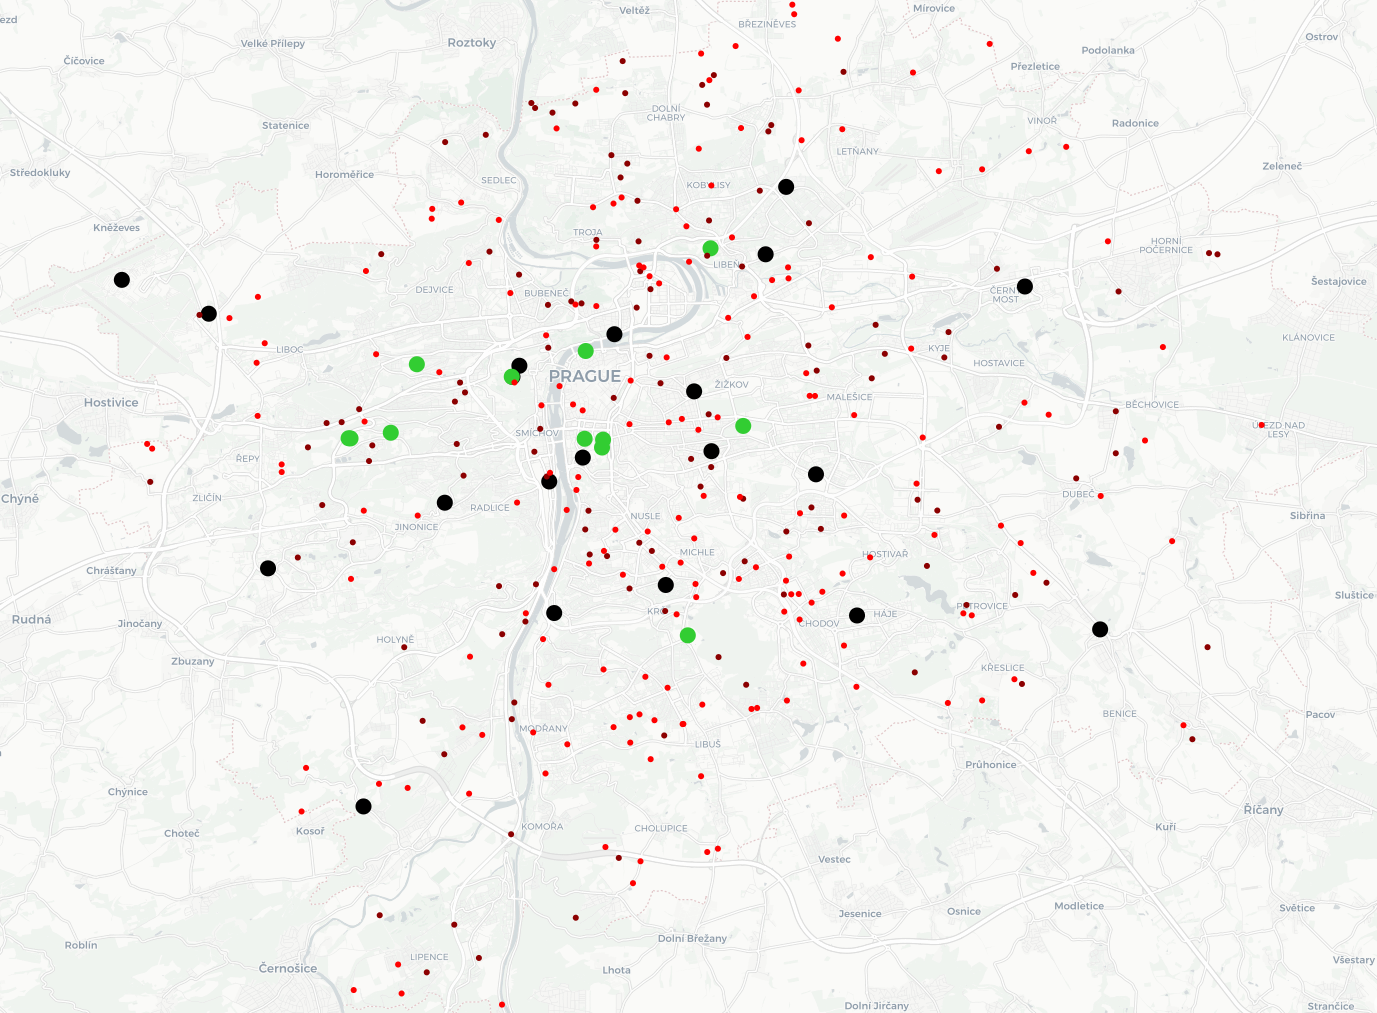
\includegraphics[width=\textwidth]{img/prague_monday_420.png}
  \centering
  \label{img:prague}
\end{figure}

Na obrázku \ref{img:prague} je znázorněno na mapě Prahy rozmístění 20 výjezdových stanic (body černé barvy), 12 nemocnic (body zelené barvy) a 300 incidentů (body červené barvy).
Tmavě červené puntíky reprezentují incidenty, které se odehrají mezi 9 a 12 hodinou.

S výše popsanou reprezentací pohotovostní služby a sady incidentů je třeba zajistit, aby simulace uměla věrohodně zjistit doby trvání příjezdů.
Připomeňme si, že simulaci používáme právě z toho důvodu, aby počet úspěšně odbavených incidentů plánem byl co nejvěrohodnější.
Věrohodnost zajistíme použitím Google API pro zjišťování těchto dob příjezdu. Konkrétně pomocí Distance Matrix API a Routes API.

V průběhu simulace je potřeba především znát následující doby příjezdů:
\begin{enumerate}
  \item z výjezdové stanice na incident,
  \item z incidentu do nemocnice,
  \item z nemocnice zpět na výjezdovou stanici.
\end{enumerate}

Simulace podporuje i tzvn. \textit{reroute}, tedy jak se záchranný tým vrací po odbavení incidentu zpět na výjezdovou stanici,
tak je povoleno, aby mohlo z aktuální lokace vyrazit na odbavování incidentu, aniž by se musela na výjezdovou stanici vrátit.

Doby příjezdů mezi výjezdovými stanicemi, incidenty a nemocnicemi si můžeme předpočítat, ale \textit{reroute} předpočítat nelze.
Můžeme si alespoň v průběhu simulování všechny spočítané doby příjezdů mezi lokacemi udržovat s přesností na desítky metrů,
aby se v budoucnu nemuselo volat Google API, což je samozřejmě pomalá operace, trvající až desítky až stovky milisekund. 

TravelDurationsRequest: 97619020/97626400


\section{Aplikace prohledávání plánů optimálními \linebreak tahy}

\section{Aplikace lokálního prohledávání}

\section{Aplikace tabu prohledávání}

\section{Aplikace simulovaného žíhání}

\section{Porovnání metod}

